
\documentclass[letterpaper,hide notes,xcolor={table,svgnames},pdftex]{beamer}
\def\showexamples{t}


%\usepackage[svgnames]{xcolor}

%% Demo talk
%\documentclass[letterpaper,notes=show]{beamer}

\usecolortheme{crane}%seahorse crane
\setbeamertemplate{navigation symbols}{}

\usetheme{MyPittsburgh}
%\usetheme{Frankfurt}

%\usepackage{tipa}

\usepackage{hyperref}
\usepackage{graphicx,xspace}
\usepackage[normalem]{ulem}

\newcommand\SF[1]{$\bigstar$\footnote{SF: #1}}

\usepackage{paratype}
\renewcommand*\familydefault{\sfdefault} %% Only if the base font of the document is to be sans serif
\usepackage[zerostyle=c]{newtxtt}
\usepackage[T1]{fontenc}

\newcounter{tmpnumSlide}
\newcounter{tmpnumNote}

\usepackage{xcolor}
\usepackage{tabu}
\definecolor{light-gray}{gray}{0.75}
\taburulecolor{light-gray}

% old question code
%\newcommand\question[1]{{$\bigstar$ \small \onlySlide{2}{#1}}}
% \newcommand\nquestion[1]{\ifdefined \presentationonly \textcircled{?} \fi \note{\par{\Large \textbf{?}} #1}}
% \newcommand\nanswer[1]{\note{\par{\Large \textbf{A}} #1}}


 \newcommand\mnote[1]{%
   \addtocounter{tmpnumSlide}{1}
   \ifdefined\showcues {~\tiny\fbox{\arabic{tmpnumSlide}}}\fi
   \note{\setlength{\parskip}{1ex}\addtocounter{tmpnumNote}{1}\textbf{\Large \arabic{tmpnumNote}:} {#1\par}}}

\newcommand\mmnote[1]{\note{\setlength{\parskip}{1ex}#1\par}}

%\newcommand\mnote[2][]{\ifdefined\handoutwithnotes {~\tiny\fbox{#1}}\fi
% \note{\setlength{\parskip}{1ex}\textbf{\Large #1:} #2\par}}

%\newcommand\mnote[2][]{{\tiny\fbox{#1}} \note{\setlength{\parskip}{1ex}\textbf{\Large #1:} #2\par}}

\newcommand\mquestion[2]{{~\color{red}\fbox{?}}\note{\setlength{\parskip}{1ex}\par{\Large \textbf{?}} #1} \note{\setlength{\parskip}{1ex}\par{\Large \textbf{A}} #2\par}\ifdefined \presentationonly \pause \fi}

\newcommand\blackboard[1]{%
\ifdefined   \showblackboard
  {#1}
  \else {\begin{center} \fbox{\colorbox{blue!30}{%
         \begin{minipage}{.95\linewidth}%
           \hspace{\stretch{1}} Some space intentionally left blank; done at the blackboard.%
         \end{minipage}}}\end{center}}%
         \fi%
}



%\newcommand\q{\tikz \node[thick,color=black,shape=circle]{?};}
%\newcommand\q{\ifdefined \presentationonly \textcircled{?} \fi}

\usepackage{listings}
\lstset{%
  keywordstyle=\bfseries,
  aboveskip=15pt,
  belowskip=15pt,
  captionpos=b,
  identifierstyle=\ttfamily,
  escapeinside={(*@}{@*)},
  stringstyle=\ttfamiliy,
  frame=lines,
  numbers=left, basicstyle=\scriptsize, numberstyle=\tiny, stepnumber=0, numbersep=2pt}

\usepackage{siunitx}
\newcommand\sius[1]{\num[group-separator = {,}]{#1}\si{\micro\second}}
\newcommand\sims[1]{\num[group-separator = {,}]{#1}\si{\milli\second}}
\newcommand\sins[1]{\num[group-separator = {,}]{#1}\si{\nano\second}}
\sisetup{group-separator = {,}, group-digits = true}

%% -------------------- tikz --------------------
\usepackage{tikz}
\usetikzlibrary{positioning}
\usetikzlibrary{arrows,backgrounds,automata,decorations.shapes,decorations.pathmorphing,decorations.markings,decorations.text}

\tikzstyle{place}=[circle,draw=blue!50,fill=blue!20,thick, inner sep=0pt,minimum size=6mm]
\tikzstyle{transition}=[rectangle,draw=black!50,fill=black!20,thick, inner sep=0pt,minimum size=4mm]

\tikzstyle{block}=[rectangle,draw=black, thick, inner sep=5pt]
\tikzstyle{bullet}=[circle,draw=black, fill=black, thin, inner sep=2pt]

\tikzstyle{pre}=[<-,shorten <=1pt,>=stealth',semithick]
\tikzstyle{post}=[->,shorten >=1pt,>=stealth',semithick]
\tikzstyle{bi}=[<->,shorten >=1pt,shorten <=1pt, >=stealth',semithick]

\tikzstyle{mut}=[-,>=stealth',semithick]

\tikzstyle{treereset}=[dashed,->, shorten >=1pt,>=stealth',thin]

\usepackage{ifmtarg}
\usepackage{xifthen}
\makeatletter
% new counter to now which frame it is within the sequence
\newcounter{multiframecounter}
% initialize buffer for previously used frame title
\gdef\lastframetitle{\textit{undefined}}
% new environment for a multi-frame
\newenvironment{multiframe}[1][]{%
\ifthenelse{\isempty{#1}}{%
% if no frame title was set via optional parameter,
% only increase sequence counter by 1
\addtocounter{multiframecounter}{1}%
}{%
% new frame title has been provided, thus
% reset sequence counter to 1 and buffer frame title for later use
\setcounter{multiframecounter}{1}%
\gdef\lastframetitle{#1}%
}%
% start conventional frame environment and
% automatically set frame title followed by sequence counter
\begin{frame}%
\frametitle{\lastframetitle~{\normalfont(\arabic{multiframecounter})}}%
}{%
\end{frame}%
}
\makeatother

\makeatletter
\newdimen\tu@tmpa%
\newdimen\ydiffl%
\newdimen\xdiffl%
\newcommand\ydiff[2]{%
    \coordinate (tmpnamea) at (#1);%
    \coordinate (tmpnameb) at (#2);%
    \pgfextracty{\tu@tmpa}{\pgfpointanchor{tmpnamea}{center}}%
    \pgfextracty{\ydiffl}{\pgfpointanchor{tmpnameb}{center}}%
    \advance\ydiffl by -\tu@tmpa%
}
\newcommand\xdiff[2]{%
    \coordinate (tmpnamea) at (#1);%
    \coordinate (tmpnameb) at (#2);%
    \pgfextractx{\tu@tmpa}{\pgfpointanchor{tmpnamea}{center}}%
    \pgfextractx{\xdiffl}{\pgfpointanchor{tmpnameb}{center}}%
    \advance\xdiffl by -\tu@tmpa%
}
\makeatother
\newcommand{\copyrightbox}[3][r]{%
\begin{tikzpicture}%
\node[inner sep=0pt,minimum size=2em](ciimage){#2};
\usefont{OT1}{phv}{n}{n}\fontsize{4}{4}\selectfont
\ydiff{ciimage.south}{ciimage.north}
\xdiff{ciimage.west}{ciimage.east}
\ifthenelse{\equal{#1}{r}}{%
\node[inner sep=0pt,right=1ex of ciimage.south east,anchor=north west,rotate=90]%
{\raggedleft\color{black!50}\parbox{\the\ydiffl}{\raggedright{}#3}};%
}{%
\ifthenelse{\equal{#1}{l}}{%
\node[inner sep=0pt,right=1ex of ciimage.south west,anchor=south west,rotate=90]%
{\raggedleft\color{black!50}\parbox{\the\ydiffl}{\raggedright{}#3}};%
}{%
\node[inner sep=0pt,below=1ex of ciimage.south west,anchor=north west]%
{\raggedleft\color{black!50}\parbox{\the\xdiffl}{\raggedright{}#3}};%
}
}
\end{tikzpicture}
}


%% --------------------

%\usepackage[excludeor]{everyhook}
%\PushPreHook{par}{\setbox0=\lastbox\llap{MUH}}\box0}

%\vspace*{\stretch{1}

%\setbox0=\lastbox \llap{\textbullet\enskip}\box0}

\setlength{\parskip}{\fill}

\newcommand\noskips{\setlength{\parskip}{1ex}}
\newcommand\doskips{\setlength{\parskip}{\fill}}

\newcommand\xx{\par\vspace*{\stretch{1}}\par}
\newcommand\xxs{\par\vspace*{2ex}\par}
\newcommand\tuple[1]{\langle #1 \rangle}
\newcommand\code[1]{{\sf \footnotesize #1}}
\newcommand\ex[1]{\uline{Example:} \ifdefined \presentationonly \pause \fi
  \ifdefined\showexamples#1\xspace\else{\uline{\hspace*{2cm}}}\fi}

\newcommand\ceil[1]{\lceil #1 \rceil}


\AtBeginSection[]
{
   \begin{frame}
       \frametitle{Outline}
       \tableofcontents[currentsection]
   \end{frame}
}



\pgfdeclarelayer{edgelayer}
\pgfdeclarelayer{nodelayer}
\pgfsetlayers{edgelayer,nodelayer,main}

\tikzstyle{none}=[inner sep=0pt]
\tikzstyle{rn}=[circle,fill=Red,draw=Black,line width=0.8 pt]
\tikzstyle{gn}=[circle,fill=Lime,draw=Black,line width=0.8 pt]
\tikzstyle{yn}=[circle,fill=Yellow,draw=Black,line width=0.8 pt]
\tikzstyle{empty}=[circle,fill=White,draw=Black]
\tikzstyle{bw} = [rectangle, draw, fill=blue!20, 
    text width=4em, text centered, rounded corners, minimum height=2em]
    
    \newcommand{\CcNote}[1]{% longname
	This work is licensed under the \textit{Creative Commons #1 3.0 License}.%
}
\newcommand{\CcImageBy}[1]{%
	\includegraphics[scale=#1]{creative_commons/cc_by_30.pdf}%
}
\newcommand{\CcImageSa}[1]{%
	\includegraphics[scale=#1]{creative_commons/cc_sa_30.pdf}%
}
\newcommand{\CcImageNc}[1]{%
	\includegraphics[scale=#1]{creative_commons/cc_nc_30.pdf}%
}
\newcommand{\CcGroupBySa}[2]{% zoom, gap
	\CcImageBy{#1}\hspace*{#2}\CcImageNc{#1}\hspace*{#2}\CcImageSa{#1}%
}
\newcommand{\CcLongnameByNcSa}{Attribution-NonCommercial-ShareAlike}


\newenvironment{changemargin}[1]{% 
  \begin{list}{}{% 
    \setlength{\topsep}{0pt}% 
    \setlength{\leftmargin}{#1}% 
    \setlength{\rightmargin}{1em}
    \setlength{\listparindent}{\parindent}% 
    \setlength{\itemindent}{\parindent}% 
    \setlength{\parsep}{\parskip}% 
  }% 
  \item[]}{\end{list}} 




\title{Lecture 17 --- Midterm Review }

\author{J. Zarnett\\
\texttt{jzarnett@uwaterloo.ca}}
\institute{Department of Electrical and Computer Engineering \\
  University of Waterloo}
\date{\today}

\begin{document}

\begin{frame}
  \titlepage
  
 \end{frame}




\begin{frame}
\frametitle{Exam Coverage}

The exam is based on material we have covered in the lectures, tutorials, and programming/weekly assignments.

Exam coverage is up to Lecture 16. More on the next slides.

Weekly assignments and programming assignments with due dates before the midterm may also appear on the exam. 

\end{frame}


\begin{frame}
\frametitle{Lecture 1: Introduction}

{\Large
\begin{itemize}
	\item Course introduction
	\item Computer development
	\item When to write a program
	\item Goals of software
\end{itemize}
}
\end{frame}

\begin{frame}
\frametitle{Lecture 2: Computer Basics / C++ Intro}

{\Large
\begin{itemize}
	\item The von Neumann architecture
	\item The memory model
	\item Execution of software
	\item How code goes from source to executable
	\item Syntax vs Semantics
	\item Software design process
	\item Elements of a program
\end{itemize}
}

\end{frame}



\begin{frame}
\frametitle{Lecture 3: Hello World \& Simple Types}

{\Large
\begin{itemize}
	\item The ``Hello World'' program
	\item The \texttt{main} entry point
	\item Writing \& compiling the program
	\item Simple types: variables
	\item Declaring and assigning variables
	\item Built-in types: numeric, char, bool
\end{itemize}
}

\end{frame}


\begin{frame}
\frametitle{Lecture 4: Console Input/Output}

{\Large
\begin{itemize}
	\item Writing to the console
	\item A bit about strings
	\item Newlines and escape sequences
	\item Console input
	\item Reading and parsing numbers
	\item Code comments
\end{itemize}
}

\end{frame}


\begin{frame}
\frametitle{Lecture 5: Expressions \& Operators}

{\Large
\begin{itemize}
	\item Operators and operands
	\item Assignment operator(s)
	\item Arithmetic operators
	\item Unary operators
	\item Order of operations (BEDMAS)
	\item Type promotion
	\item Explicit type conversion
\end{itemize}
}

\end{frame}



\begin{frame}
\frametitle{Lecture 6: Relational \& Bitwise Operators}

{\Large
\begin{itemize}
	\item Relational operators
	\item Numerical comparisons
	\item Boolean logic (AND/OR/NOT)
	\item Short-circuit evaluation
	\item Bitwise operators
\end{itemize}
}

\end{frame}



\begin{frame}
\frametitle{Lecture 7: Selection Statements}

{\Large
\begin{itemize}
	\item The \texttt{if} statement
	\item The \texttt{if-else} statement
	\item All together now: \texttt{if/else if/else}
	\item The \texttt{switch} statement	
\end{itemize}
}

\end{frame}

\begin{frame}
\frametitle{Lecture 8: Loops}

{\Large
\begin{itemize}
	\item Iteration statements
	\item Pre- and posttest loops
	\item The \texttt{while} loop
	\item The \texttt{break} statement
	\item The \texttt{continue} statement
	\item \texttt{do-while} loops
	
\end{itemize}
}

\end{frame}

\begin{frame}
\frametitle{Lecture 9: More Loops}

{\Large
\begin{itemize}
	\item The \texttt{for} loop
	\item Variations on the \texttt{for}
	\item Use of \texttt{break} and \texttt{continue}
\end{itemize}
}

\end{frame}


\begin{frame}
\frametitle{Lecture 10: Enumerated Types \& Structures}

{\Large
\begin{itemize}
	\item Defining an enumerated type
	\item The \texttt{struct}
	\item The dot operator
	\item Structure assignment and nesting
\end{itemize}
}

\end{frame}

\begin{frame}
\frametitle{Lecture 11: Arrays}

{\Large
\begin{itemize}
	\item Defining arrays
	\item Declaring arrays
	\item Initializing arrays
	\item The \texttt{[~]} operator
	\item Dynamic array allocation
	\item Array length
	
\end{itemize}
}

\end{frame}


\begin{frame}
\frametitle{Lecture 12: More About Arrays}

{\Large
\begin{itemize}
%	\item The \texttt{foreach} loop
	\item Strings as arrays
	\item Multi-dimensional arrays
\end{itemize}
}

\end{frame}


\begin{frame}
\frametitle{Lecture 13: Functions}

{\Large
\begin{itemize}
	\item Mathematical functions
	\item Function signatures
	\item Formal and actual parameters
	\item Calling a function
	\item Defining a function
	\item Function execution semantics
	\item Return types
	\item \texttt{void} functions
	
	
\end{itemize}
}

\end{frame}

\begin{frame}
\frametitle{Lecture 14: More About Functions}

{\Large
\begin{itemize}
	\item Structuring the program with functions	
	\item Documenting: pre/postconditions
	\item Variable scope
	\item Function overloading
\end{itemize}
}

\end{frame}

\begin{frame}
\frametitle{Lecture 15: Parameter Passing}

{\Large
\begin{itemize}
	\item Optional parameters
	\item Pass by value, pass by reference
	\item Values, references, and  arrays	
\end{itemize}
}

\end{frame}


\begin{frame}
\frametitle{Lecture 16: Recursive Functions}

{\Large
\begin{itemize}
	\item What is recursion?
	\item Recursion vs iteration
	\item Thinking recursively
	
\end{itemize}
}

\end{frame}

%%%%%%%%%%%%%%%


\begin{frame}
\frametitle{How to Prepare}

How to prepare for the midterm exam:

\begin{enumerate}
	\item Review lecture notes and slides.
	\item Review the tutorial slides.
	\item Understand your programming assignment solutions.
	\item Try old exams.
	\item Do textbook questions for extra practice.
	\item Ask for extra help (we have many TAs and instructors).
\end{enumerate}

\end{frame}

\begin{frame}
\frametitle{Exam Tips}

Tips for the Exam:

\begin{enumerate}
	\item Take the time to read the question carefully.
	\item You can use point form instead of full sentences in answers if it's not a code question.
	\item Don't leave questions blank - Nothing on the page = 0 marks.
	\item Do the questions you know (or find easy) first, then move on to more challenging ones.
	\item Keep an eye on the time.
	\item Review your work before the end of the exam.
	\item Sleep the night before (all nighters are bad).
	
\end{enumerate}

\end{frame}


\begin{frame}
\frametitle{About Grades}

\begin{center}
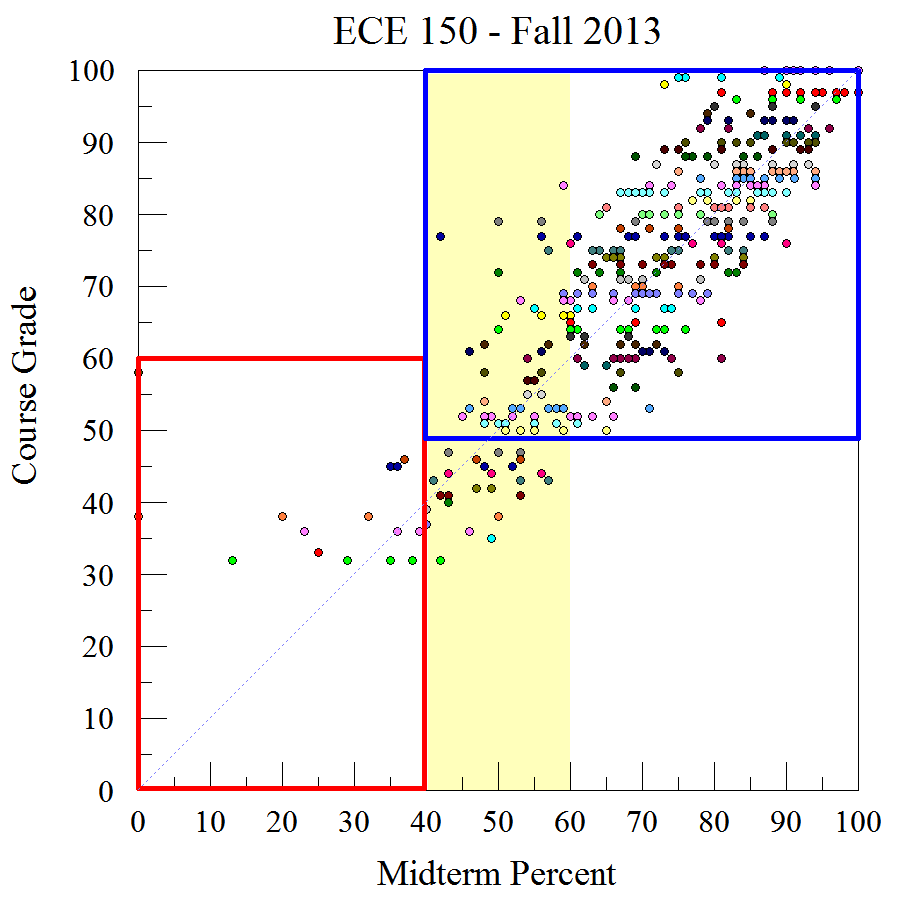
\includegraphics[width=0.7\textwidth]{images/2013-midterm-plot.png}
\end{center}

\end{frame}

\begin{frame}
\frametitle{About Grades}

\begin{center}
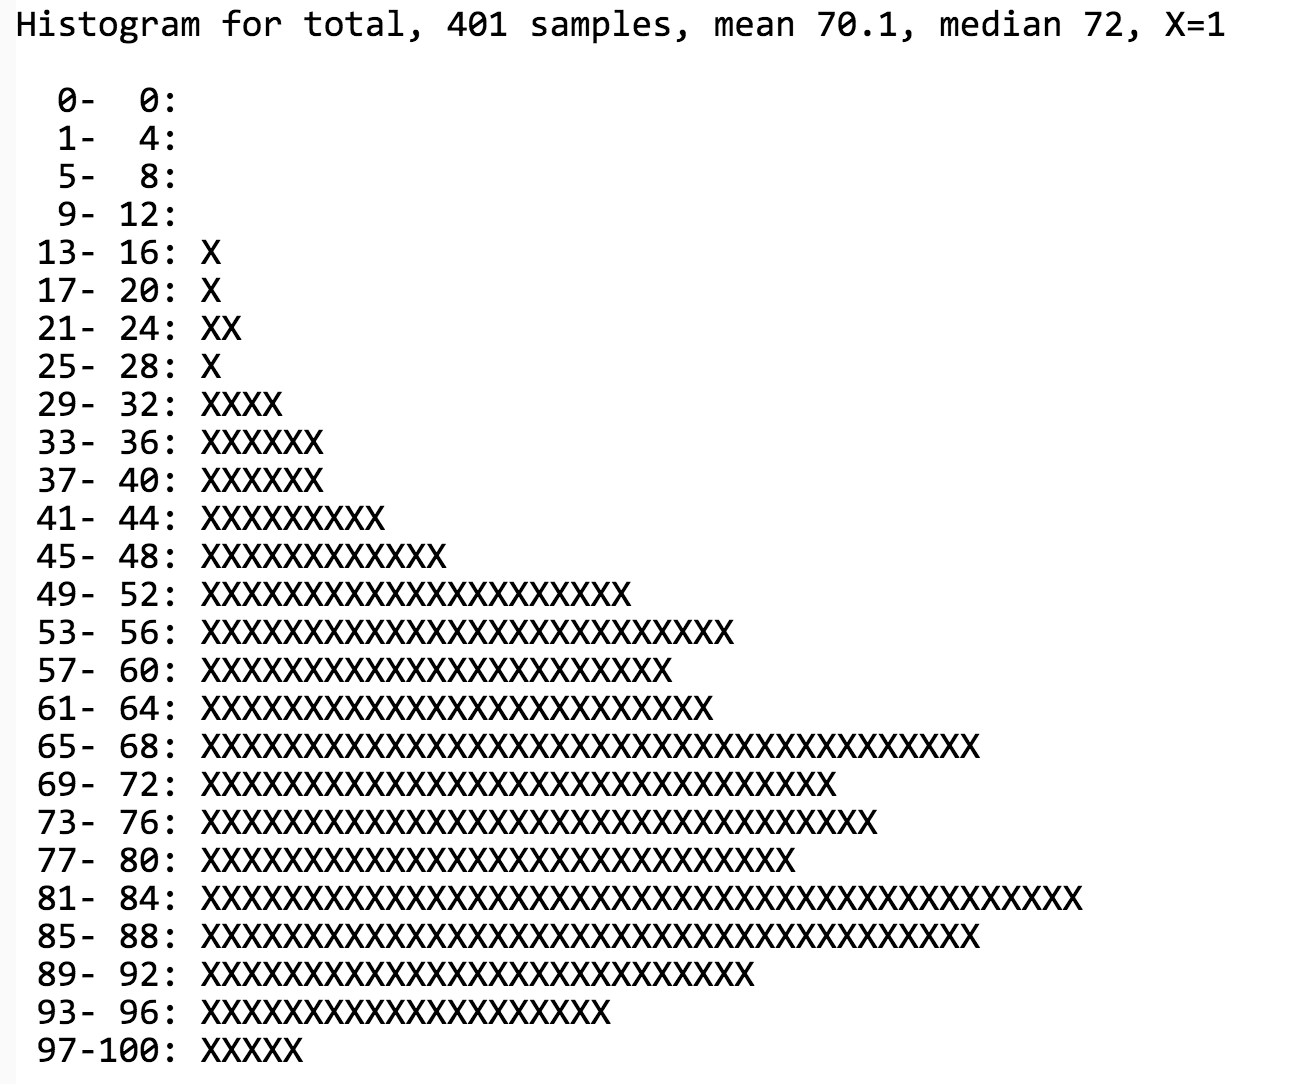
\includegraphics[width=0.7\textwidth]{images/2013-midterm-histogram.png}
\end{center}

\end{frame}

\begin{frame}
\frametitle{About Grades}

No midterm grades can be released until midterm week is over.

We will try to mark quickly, but we can't promise a specific date.\\
\quad\quad Important note: asking does not make marking faster.

\end{frame}


\end{document}

